\documentclass[12pt,]{article}
\usepackage{lmodern}
\usepackage{amssymb,amsmath}
\usepackage{ifxetex,ifluatex}
\usepackage{fixltx2e} % provides \textsubscript
\ifnum 0\ifxetex 1\fi\ifluatex 1\fi=0 % if pdftex
  \usepackage[T1]{fontenc}
  \usepackage[utf8]{inputenc}
\else % if luatex or xelatex
  \ifxetex
    \usepackage{mathspec}
  \else
    \usepackage{fontspec}
  \fi
  \defaultfontfeatures{Ligatures=TeX,Scale=MatchLowercase}
    \setmainfont[]{Times New Roman}
\fi
% use upquote if available, for straight quotes in verbatim environments
\IfFileExists{upquote.sty}{\usepackage{upquote}}{}
% use microtype if available
\IfFileExists{microtype.sty}{%
\usepackage{microtype}
\UseMicrotypeSet[protrusion]{basicmath} % disable protrusion for tt fonts
}{}
\usepackage[margin=2.54cm]{geometry}
\usepackage{hyperref}
\hypersetup{unicode=true,
            pdftitle={Examining the Hydrologic Properties of the Missouri River Basin},
            pdfauthor={Rachel Bash, Keqi He, Caroline Watson, and Haoyu Zhang},
            pdfborder={0 0 0},
            breaklinks=true}
\urlstyle{same}  % don't use monospace font for urls
\usepackage{color}
\usepackage{fancyvrb}
\newcommand{\VerbBar}{|}
\newcommand{\VERB}{\Verb[commandchars=\\\{\}]}
\DefineVerbatimEnvironment{Highlighting}{Verbatim}{commandchars=\\\{\}}
% Add ',fontsize=\small' for more characters per line
\usepackage{framed}
\definecolor{shadecolor}{RGB}{248,248,248}
\newenvironment{Shaded}{\begin{snugshade}}{\end{snugshade}}
\newcommand{\AlertTok}[1]{\textcolor[rgb]{0.94,0.16,0.16}{#1}}
\newcommand{\AnnotationTok}[1]{\textcolor[rgb]{0.56,0.35,0.01}{\textbf{\textit{#1}}}}
\newcommand{\AttributeTok}[1]{\textcolor[rgb]{0.77,0.63,0.00}{#1}}
\newcommand{\BaseNTok}[1]{\textcolor[rgb]{0.00,0.00,0.81}{#1}}
\newcommand{\BuiltInTok}[1]{#1}
\newcommand{\CharTok}[1]{\textcolor[rgb]{0.31,0.60,0.02}{#1}}
\newcommand{\CommentTok}[1]{\textcolor[rgb]{0.56,0.35,0.01}{\textit{#1}}}
\newcommand{\CommentVarTok}[1]{\textcolor[rgb]{0.56,0.35,0.01}{\textbf{\textit{#1}}}}
\newcommand{\ConstantTok}[1]{\textcolor[rgb]{0.00,0.00,0.00}{#1}}
\newcommand{\ControlFlowTok}[1]{\textcolor[rgb]{0.13,0.29,0.53}{\textbf{#1}}}
\newcommand{\DataTypeTok}[1]{\textcolor[rgb]{0.13,0.29,0.53}{#1}}
\newcommand{\DecValTok}[1]{\textcolor[rgb]{0.00,0.00,0.81}{#1}}
\newcommand{\DocumentationTok}[1]{\textcolor[rgb]{0.56,0.35,0.01}{\textbf{\textit{#1}}}}
\newcommand{\ErrorTok}[1]{\textcolor[rgb]{0.64,0.00,0.00}{\textbf{#1}}}
\newcommand{\ExtensionTok}[1]{#1}
\newcommand{\FloatTok}[1]{\textcolor[rgb]{0.00,0.00,0.81}{#1}}
\newcommand{\FunctionTok}[1]{\textcolor[rgb]{0.00,0.00,0.00}{#1}}
\newcommand{\ImportTok}[1]{#1}
\newcommand{\InformationTok}[1]{\textcolor[rgb]{0.56,0.35,0.01}{\textbf{\textit{#1}}}}
\newcommand{\KeywordTok}[1]{\textcolor[rgb]{0.13,0.29,0.53}{\textbf{#1}}}
\newcommand{\NormalTok}[1]{#1}
\newcommand{\OperatorTok}[1]{\textcolor[rgb]{0.81,0.36,0.00}{\textbf{#1}}}
\newcommand{\OtherTok}[1]{\textcolor[rgb]{0.56,0.35,0.01}{#1}}
\newcommand{\PreprocessorTok}[1]{\textcolor[rgb]{0.56,0.35,0.01}{\textit{#1}}}
\newcommand{\RegionMarkerTok}[1]{#1}
\newcommand{\SpecialCharTok}[1]{\textcolor[rgb]{0.00,0.00,0.00}{#1}}
\newcommand{\SpecialStringTok}[1]{\textcolor[rgb]{0.31,0.60,0.02}{#1}}
\newcommand{\StringTok}[1]{\textcolor[rgb]{0.31,0.60,0.02}{#1}}
\newcommand{\VariableTok}[1]{\textcolor[rgb]{0.00,0.00,0.00}{#1}}
\newcommand{\VerbatimStringTok}[1]{\textcolor[rgb]{0.31,0.60,0.02}{#1}}
\newcommand{\WarningTok}[1]{\textcolor[rgb]{0.56,0.35,0.01}{\textbf{\textit{#1}}}}
\usepackage{graphicx,grffile}
\makeatletter
\def\maxwidth{\ifdim\Gin@nat@width>\linewidth\linewidth\else\Gin@nat@width\fi}
\def\maxheight{\ifdim\Gin@nat@height>\textheight\textheight\else\Gin@nat@height\fi}
\makeatother
% Scale images if necessary, so that they will not overflow the page
% margins by default, and it is still possible to overwrite the defaults
% using explicit options in \includegraphics[width, height, ...]{}
\setkeys{Gin}{width=\maxwidth,height=\maxheight,keepaspectratio}
\IfFileExists{parskip.sty}{%
\usepackage{parskip}
}{% else
\setlength{\parindent}{0pt}
\setlength{\parskip}{6pt plus 2pt minus 1pt}
}
\setlength{\emergencystretch}{3em}  % prevent overfull lines
\providecommand{\tightlist}{%
  \setlength{\itemsep}{0pt}\setlength{\parskip}{0pt}}
\setcounter{secnumdepth}{5}
% Redefines (sub)paragraphs to behave more like sections
\ifx\paragraph\undefined\else
\let\oldparagraph\paragraph
\renewcommand{\paragraph}[1]{\oldparagraph{#1}\mbox{}}
\fi
\ifx\subparagraph\undefined\else
\let\oldsubparagraph\subparagraph
\renewcommand{\subparagraph}[1]{\oldsubparagraph{#1}\mbox{}}
\fi

%%% Use protect on footnotes to avoid problems with footnotes in titles
\let\rmarkdownfootnote\footnote%
\def\footnote{\protect\rmarkdownfootnote}

%%% Change title format to be more compact
\usepackage{titling}

% Create subtitle command for use in maketitle
\providecommand{\subtitle}[1]{
  \posttitle{
    \begin{center}\large#1\end{center}
    }
}

\setlength{\droptitle}{-2em}

  \title{Examining the Hydrologic Properties of the Missouri River Basin}
    \pretitle{\vspace{\droptitle}\centering\huge}
  \posttitle{\par}
  \subtitle{\url{https://github.com/cwatson1013/Hydrologic_Data_Analysis_Final_Proj}}
  \author{Rachel Bash, Keqi He, Caroline Watson, and Haoyu Zhang}
    \preauthor{\centering\large\emph}
  \postauthor{\par}
    \date{}
    \predate{}\postdate{}
  
\usepackage{booktabs}
\usepackage{longtable}
\usepackage{array}
\usepackage{multirow}
\usepackage{wrapfig}
\usepackage{float}
\usepackage{colortbl}
\usepackage{pdflscape}
\usepackage{tabu}
\usepackage{threeparttable}
\usepackage{threeparttablex}
\usepackage[normalem]{ulem}
\usepackage{makecell}
\usepackage{xcolor}

\begin{document}
\maketitle
\begin{abstract}
The Missouri River provides critical water resources that drives the
region's agriculture, industry, and ecosystems. This is a region that
experiences surface water variability, characterized by damaging floods
and severe droughts, greatly impacting the agricultural production of
the area. It is reported that a serious flood disaster occurred in the
lower Missouri River in the spring of 2019 and the Missouri River
experienced severe drought in 2012-2013. This project highlights the
changes in stream flow and water quality over time, and identifies key
characteristics of the river. Twenty two sites across the lower Missouri
River Basin were examined in order to get a fuller picture of the
Missouri River and its tributaries over time. By analyzing the trend of
the Missouri River discharge, we can predict future changes in the
Missouri River flow to provide a reference for water resources
management. In addition, we focus on the stream flow and water quality
of Missouri River during March to July, 2019 to see how discharge
influence the water quality and what can be done to keep the water in
the Missouri River in good quality.
\end{abstract}

\textless Information in these brackets are used for annotating the
RMarkdown file. They will not appear in the final version of the PDF
document\textgreater{}

\newpage
\tableofcontents 
\newpage
\listoftables 
\newpage
\listoffigures 
\newpage

\textless Note: set up autoreferencing for figures and tables in your
document\textgreater{}

\hypertarget{research-question-and-rationale}{%
\section{Research Question and
Rationale}\label{research-question-and-rationale}}

\textless Paragraph detailing the rationale for your analysis. What is
the significant application and/or interest in this topic? Connect to
environmental topic(s)/challenge(s).\textgreater{}

\textless Paragraph detailing your research question(s) and goals. What
do you want to find out? Include a sentence (or a few) on the dataset
you are using to answer this question - just enough to give your reader
an idea of where you are going with the analysis.\textgreater{}

The Missouri River is the largest river in North America (2,540 miles)
and has the second largest watershed (529,000 mi\textsuperscript{2}/339
acres, U.S.-Canada). Its watershed covers portions of ten states, which
account for approximately one-sixth of the continental United States, as
well as a small part of Canada. The headwater is located in the
Bitterroot Mountains River of northwestern Wyoming and southwestern
Montana. The watershed is home to around 12 million people in 1990, and
has been inhabited by indigenous people for millennia. Demands for
managing the river for the benefit of human livelihood has resulted in
drastic modification in the river and the floodplains. Numerous
reservoirs and dams have been constructed, of which six major dams were
built on the mainstream, following the Pick-Sloan Plan in 1944. Now, the
river is used intensively in multiple ways, including municipal,
agricultural, hydropower, recreation, flood control etc. \newline Within
the 328 million acres of the basin's total area in the United States,
95\% is related to agricultural uses, while the rest dedicated for
recreation, fish and wildlife, and urban. More than half of the total is
pasture and range grassland primarily for grazing, and cropland consists
of almost 104 million acres, which is 32\% of the whole basin. Irrigated
land comprises 7.4 million acres, and 6.9 million acres are intensively
cropped. Water bodies, on the other hand, cover 3.9 million acres. In
spite of the low proportion of water areas (1.2\%), they are the pivotal
foundation for agricultural or other usages, and thus critical to the
whole region's economy. \newline Along with the agricultural, urban, and
industrial development in the region is nutrient loading and enrichment
in water bodies, especially for nitrogen (N) and phosphorus (P). Unlike
other regions, agricultural input through fertilizer is the predominant
anthropogenic source for nutrient in water bodies in the whole basin.
Regardless of the major anthropogenic source, nutrient enrichment is
considered nationally as one of the leading factors for water quality
impairment. According to USEPA 303(d) lists, more than 160 stream
reaches, lakes, or reservoirs were reported by USEPA to be
nutrient-related impaired in 2006. \newline In addition to change in
nutrient concentration, discharge appears to be highly variable in the
basin, and both severe drought and flooding events occurred in the basin
in the past. For example, in the spring and summer of 2011, an
unprecedented flooding event caused over \$2 billion damage FEMA
disaster declaration was made in all states along the Missouri River.
Subsequently, in 2012, a drought even struck the Central Great Plain,
including the basin, and inflicted at least \$12 billion of loss before
July, 2012. Recently, another flooding event occurred in the spring of
2019. Given all the background information above, we would like to know
the current state of Missouri River and its tributaries, with a focus on
the changing pattern in discharge and nutrient. We are interested in how
the dramatic change in discharge (i.e.~water quantity) could potentially
interact with nutrient enrichment (i.e.~water quality). Also, we
examined a few specific flooding events, during which changes in both
water quality and quantity were well recorded, so that we could make
concrete inference on the interplay between quantity and quality.
Finally, based on the pattern in the past and the best model we could
fit, we attempted to predict the likely future conditions and trends in
the Missouri River Basin. To achieve these goals, we retrieved data on
water quantity, water quality (N, P concentrations), pH, coliform
concentrations from USGS National Water Information System, using the
package \texttt{dataRetrieval}.

\newpage

\hypertarget{dataset-information}{%
\section{Dataset Information}\label{dataset-information}}

\textless Information on how the dataset for this analysis were
collected, the data contained in the dataset, and any important pieces
of information that are relevant to your analyses. This section should
contain much of same information as the README file for the dataset but
formatted in a way that is more narrative.\textgreater{}

The data we are analyzing comes from the United States Geological Survey
(USGS) database called the National Water Information System interface,
or NWIS. We pulled data from the interface using the R package
\texttt{dataRetrieval}. Because we are interested in the lower Missouri
River basin, we pulled sites from each HUC4 subbasin from 1020 to 1030
(see Figure below). We chose these subbasins because they had a variety
of tributaries that all flowed into the Missouri River, and we wanted a
variety of river sizes and lengths. We filtered these subbasin queries
to only show us sites that had discharge, nitrogen, and phosphorus data.
Once we found the sites with all of this data, we chose 2 sites from
each HUC sub basin as our 22 ``best sites''. Our best sites had the
overall best time period range for all of our ``must have'' variables.

Only seven sites within our HUC subbasin boundary contained any high
frequency discharge and nitrogen data. Therefore, we also looked at
these 7 sites in order to do analyses and answer our research question
about flooding.

After doing initial data wrangling and analysis on our 22 ``best
sites'', we decided to pare it down further and only do subsequent
analyses on \textbf{10} sites. While we initially wanted to look at many
sites that were varied in size and location, we determined that it was
too many to look at and draw relevant conclusions from.

We have three main datasets:

\begin{itemize}
\item
  The daily values dataset with our 22 ``best sites''
\item
  The water quality dataset with our 22 ``best sites'', with only six
  sites that had total coliform data.
\item
  The high freqency dataset with 7 sites that contain both high freqency
  discharge and high frequency nitrogen data.
\end{itemize}

\textless Add a table that summarizes your data structure. This table
can be made in markdown text or inserted as a \texttt{kable} function in
an R chunk. If the latter, do not include the code used to generate your
table.\textgreater{}

\textless C will do data table for water quality and daily values, R
will do for high freq\textgreater{}

\begin{landscape}\begin{table}[!h]

\caption{\label{tab:unnamed-chunk-3}Summary of Daily Value Data at 22 sites in the
      Missouri River Basin}
\centering
\resizebox{\linewidth}{!}{
\begin{tabular}[t]{l|l|l|l|l|l|l|l|l|l|l|l|l|l|l|l|l|l|l|l|l|l|l|l|l|l|l|l|l|l|l|l|l|l|l|l|l|l|l}
\hline
  &       X & agency\_cd &    site\_no &         Date &   Discharge & Approval.Code &    parm\_cd &   sample\_tm & sample\_end\_dt & sample\_end\_tm & sample\_start\_time\_datum\_cd & tm\_datum\_rlbty\_cd &   coll\_ent\_cd & medium\_cd &     project\_cd & aqfr\_cd &  tu\_id & body\_part\_id &  hyd\_cond\_cd &  samp\_type\_cd &  hyd\_event\_cd &                              sample\_lab\_cm\_tx & remark\_cd &   result\_va &  val\_qual\_tx &    meth\_cd &  dqi\_cd &   rpt\_lev\_va &  rpt\_lev\_cd & lab\_std\_va & prep\_set\_no & prep\_dt &    anl\_set\_no &     anl\_dt &                                                                                                                               result\_lab\_cm\_tx &    anl\_ent\_cd &             startDateTime &            parameter\\
\hline
\rowcolor{gray!6}   & Min.   :     1 & USGS:658650 & Min.   :6609500 & 2009-10-20:    36 & Min.   :     0 & A      :618881 & Min.   : 60.00 & 11:00  :  1108 & Mode:logical & 14:15  :     8 & CDT :  8481 & K   :  5636 & USGS-WRD:  9272 & WS  : 13164 & NAWQA-SWS:   879 & Mode:logical & Mode:logical & Mode:logical & 9      :  5662 & 9      : 11792 & 9      : 11673 & tech samples                         :    90 & <   :   470 & Min.   :  0.0 & d      :   426 & ALGOR  :  4992 & A   :  6906 & Min.   :0.0 & DLDQC :   614 & Mode:logical & Mode:logical & Mode:logical & KJNT254A:    12 & Min.   :20010918 & The parameter 00665 was swapped from labcode 2333 to labcode 2759                                                                     :   160 & USGSNWQL:  2213 & 2018-05-08 10:30:00:     6 & Discharge       :645422\\
\hline
 & 1st Qu.:164663 & NA & 1st Qu.:6800000 & 2009-11-18:    36 & 1st Qu.:   154 & A e    : 21858 & 1st Qu.: 60.00 & 10:30  :   883 & NA's:658650 & 11:15  :     6 & CST :  4747 & T   :  7592 & USGS-NEL:  1051 & WSQ :    64 & 462900300:   689 & NA's:658650 & NA's:658650 & NA's:658650 & A      :  3373 & A      :   813 & Z      :   863 & tech sample                          :    75 & E   :    71 & 1st Qu.:  0.3 & oc     :   266 & KJ009  :  2579 & R   :  5574 & 1st Qu.:0.0 & LRL   :  1226 & NA's:658650 & NA's:658650 & NA's:658650 & KJNT135A:    11 & 1st Qu.:20070427 & The parameter 00665 was swapped from labcode 2333 to labcode 1984 because the result from labcode 2333 exceeded the calibration range.:    79 & NA's    :656437 & 1975-01-15 11:20:00:     4 & Total Nitrogen  :  6207\\
\hline
\rowcolor{gray!6}   & Median :329326 & NA & Median :6856600 & 1982-03-09:    35 & Median :   756 & P      :  4304 & Median : 60.00 & 10:00  :   831 & NA & 04:15  :     4 & NA's:645422 & NA's:645422 & USGSKSWC:   596 & NA's:645422 & 463106100:   649 & NA & NA & NA & 5      :  1397 & 7      :   515 & J      :   292 & tech sample;no sampling method given :    25 & NA's:658109 & Median :  0.7 & n      :    56 & CL084  :   701 & S   :   748 & Median :0.0 & LT-MDL:  1059 & NA & NA & NA & KJNT200A:    10 & Median :20120366 & The parameter 00665 was swapped from labcode 2333 to labcode 2759 because the result from labcode 2333 exceeded the calibration range.:    77 & NA & 1975-02-12 10:30:00:     4 & Total Phosphorus:  7021\\
\hline
 & Mean   :329326 & NA & Mean   :6828931 & 1980-08-12:    34 & Mean   : 10226 & P e    :   246 & Mean   : 71.54 & 12:00  :   750 & NA & 05:00  :     4 & NA & NA & USGS    :   517 & NA & 861100399:   542 & NA & NA & NA & 4      :  1235 & H      :    94 & 7      :   151 & tech samples;cross section from churn:    22 & NA & Mean   :  1.7 & doc    :    47 & CL021  :   609 & NA's:645422 & Mean   :0.0 & MRL   :    21 & NA & NA & NA & KJNT021A:     9 & Mean   :20111394 & Report level code updated Oct., Nov. 2015. Reference: NWQL TM 2015.02 (RLC: LT-MDL => DLDQC)                                          :    23 & NA & 1975-03-11 10:50:00:     4 & NA\\
\hline
\rowcolor{gray!6}   & 3rd Qu.:493988 & NA & 3rd Qu.:6892350 & 2017-07-25:    34 & 3rd Qu.:  4670 & P Ice  :    79 & 3rd Qu.: 60.00 & 11:30  :   747 & NA & 06:15  :     4 & NA & NA & USGSMOLS:   186 & NA & 463100300:   498 & NA & NA & NA & 8      :   692 & 5      :     8 & B      :   149 & BOTTLES OK                           :    18 & NA & 3rd Qu.:  2.2 & @d     :    11 & AKP01  :   411 & NA & 3rd Qu.:0.0 & NA's  :655730 & NA & NA & NA & KJNT023A:     9 & 3rd Qu.:20151101 & The holding time for the processing of this sample has been exceeded                                                                  :    12 & NA & 1975-07-22 10:00:00:     4 & NA\\
\hline
 & Max.   :658650 & NA & Max.   :6934500 & 1979-06-13:    33 & Max.   :739000 & (Other):    54 & Max.   :665.00 & (Other):  8903 & NA & (Other):    98 & NA & NA & (Other) :   188 & NA & (Other)  :  6154 & NA & NA & NA & (Other):   869 & (Other):     6 & (Other):   100 & (Other)                              :  3975 & NA & Max.   :100.0 & (Other):    62 & (Other):   392 & NA & Max.   :0.8 & NA & NA & NA & NA & (Other) :  2869 & Max.   :20191023 & (Other)                                                                                                                               :    28 & NA & (Other)            : 13200 & NA\\
\hline
\rowcolor{gray!6}   & NA & NA & NA & (Other)   :658442 & NA's   :13360 & NA's   : 13228 & NA & NA's   :645428 & NA & NA's   :658526 & NA & NA & NA's    :646840 & NA & NA's     :649239 & NA & NA & NA & NA's   :645422 & NA's   :645422 & NA's   :645422 & NA's                                 :654445 & NA & NA's   :645422 & NA's   :657782 & NA's   :648966 & NA & NA's   :655730 & NA & NA & NA & NA & NA's    :655730 & NA's   :655730 & NA's                                                                                                                                  :658271 & NA & NA's               :645428 & NA\\
\hline
\end{tabular}}
\end{table}
\end{landscape}

\begin{landscape}\begin{table}[!h]

\caption{\label{tab:unnamed-chunk-4}Summary of Water Quality Data in the
      Missouri River Basin}
\centering
\resizebox{\linewidth}{!}{
\begin{tabular}[t]{l|l|l|l|l|l|l|l|l|l|l|l|l|l|l|l|l|l|l|l|l|l|l|l|l|l|l|l|l|l|l|l|l|l|l|l|l|l}
\hline
  &       X & agency\_cd &   site\_no &      Date & X\_00060\_00003 & X\_00060\_00003\_cd &   parm\_cd &   sample\_tm & sample\_end\_dt & sample\_end\_tm & sample\_start\_time\_datum\_cd & tm\_datum\_rlbty\_cd &   coll\_ent\_cd & medium\_cd &     project\_cd & aqfr\_cd &     tu\_id &  body\_part\_id &  hyd\_cond\_cd &  samp\_type\_cd &  hyd\_event\_cd &                              sample\_lab\_cm\_tx & remark\_cd &   result\_va &  val\_qual\_tx &    meth\_cd &  dqi\_cd &   rpt\_lev\_va &  rpt\_lev\_cd & lab\_std\_va & prep\_set\_no & prep\_dt &    anl\_set\_no &     anl\_dt &                                                                                                                               result\_lab\_cm\_tx &    anl\_ent\_cd &             startDateTime\\
\hline
\rowcolor{gray!6}   & Min.   :     1 & USGS:668800 & Length:668800 & Min.   :1899-10-01 & Min.   :     0 & A      :618881 & Length:668800 & 11:00  :  1819 & Mode:logical & 14:15  :    12 & CDT : 14622 & K   :  8908 & USGS-WRD: 15396 & BI  :    11 & NAWQA-SWS:  1411 & Mode:logical & Min.   :0 & Min.   :59.0 & 9      :  9726 & 9      : 20163 & 9      : 19933 & tech samples                         :   149 & <   :   472 & Min.   :     0.0 & d      :   426 & ALGOR  :  4994 & A   : 12661 & Min.   :0.0 & DLDQC :   616 & Mode:logical & Mode:logical & Mode:logical & KJNT254A:    12 & Min.   :20010918 & The parameter 00665 was swapped from labcode 2333 to labcode 2759                                                                     :   160 & USGS-WRD:  2206 & 2018-05-08 10:30:00:     9\\
\hline
 & 1st Qu.:167201 & NA & Class :character & 1st Qu.:1957-05-09 & 1st Qu.:   154 & A e    : 21858 & Class :character & 10:30  :  1402 & NA's:668800 & 11:15  :    10 & CST :  8672 & T   : 14386 & USGS-NEL:  1690 & BP  :    41 & 462900300:  1089 & NA's:668800 & 1st Qu.:0 & 1st Qu.:59.0 & A      :  6963 & A      :  2127 & Z      :  2203 & tech sample                          :   127 & >   :     1 & 1st Qu.:     0.6 & oc     :   266 & KJ009  :  2581 & R   :  9500 & 1st Qu.:0.0 & LRL   :  1226 & NA's:668800 & NA's:668800 & NA's:668800 & KJNT135A:    11 & 1st Qu.:20070428 & The parameter 00665 was swapped from labcode 2333 to labcode 1984 because the result from labcode 2333 exceeded the calibration range.:    79 & USGSKSWC:   392 & 1979-06-13 11:00:00:     7\\
\hline
\rowcolor{gray!6}   & Median :334400 & NA & Mode  :character & Median :1979-10-01 & Median :   756 & P      :  4388 & Mode  :character & 10:00  :  1390 & NA & 05:00  :     7 & NA's:645506 & NA's:645506 & USGSKSWC:   988 & ON  :    26 & 463106100:   991 & NA & Median :0 & Median :94.0 & 5      :  2201 & 7      :   831 & J      :   530 & tech sample;no sampling method given :    50 & A   :    21 & Median :     3.8 & n      :    56 & PROBE  :  2013 & S   :  1133 & Median :0.0 & LT-MDL:  1059 & NA & NA & NA & KJNT200A:    10 & Median :20120404 & The parameter 00665 was swapped from labcode 2333 to labcode 2759 because the result from labcode 2333 exceeded the calibration range.:    77 & USGSNWQL:  2215 & 1975-01-15 11:20:00:     6\\
\hline
 & Mean   :334400 & NA & NA & Mean   :1977-11-11 & Mean   : 10227 & P e    :   246 & NA & 12:00  :  1277 & NA & 04:15  :     6 & NA & NA & USGS    :   805 & SB  :     8 & 463100300:   853 & NA & Mean   :0 & Mean   :81.2 & 4      :  1939 & H      :   149 & 7      :   248 & Billed FY19.                         :    48 & E   :   113 & Mean   :    88.9 & doc    :    47 & CL084  :   701 & NA's:645506 & Mean   :0.0 & MRL   :    21 & NA & NA & NA & KJNT021A:     9 & Mean   :20111448 & Report level code updated Oct., Nov. 2015. Reference: NWQL TM 2015.02 (RLC: LT-MDL => DLDQC)                                          :    23 & NA's    :663987 & 1975-02-12 10:30:00:     6\\
\hline
\rowcolor{gray!6}   & 3rd Qu.:501600 & NA & NA & 3rd Qu.:2000-03-12 & 3rd Qu.:  4670 & P Ice  :    79 & NA & 11:30  :  1232 & NA & 06:15  :     6 & NA & NA & USGSMOLS:   290 & WS  : 23094 & 861100399:   813 & NA & 3rd Qu.:0 & 3rd Qu.:94.0 & 8      :  1089 & 5      :    15 & B      :   224 & tech samples;cross section from churn:    33 & NA's:668193 & 3rd Qu.:     8.0 & @d     :    11 & EL003  :   678 & NA & 3rd Qu.:0.0 & NA's  :665878 & NA & NA & NA & KJNT023A:     9 & 3rd Qu.:20151102 & The holding time for the processing of this sample has been exceeded                                                                  :    12 & NA & 1975-03-11 10:50:00:     6\\
\hline
 & Max.   :668800 & NA & NA & Max.   :2019-11-10 & Max.   :739000 & (Other):    54 & NA & (Other): 15541 & NA & (Other):   150 & NA & NA & (Other) :   282 & WSQ :   114 & (Other)  : 10401 & NA & Max.   :0 & Max.   :94.0 & (Other):  1376 & (Other):     9 & (Other):   156 & (Other)                              :  6153 & NA & Max.   :400000.0 & (Other):    67 & (Other):  1566 & NA & Max.   :0.8 & NA & NA & NA & NA & (Other) :  2871 & Max.   :20191023 & (Other)                                                                                                                               :    29 & NA & (Other)            : 22627\\
\hline
\rowcolor{gray!6}   & NA & NA & NA & NA & NA's   :23426 & NA's   : 23294 & NA & NA's   :646139 & NA & NA's   :668609 & NA & NA & NA's    :649349 & NA's:645506 & NA's     :653242 & NA & NA's   :668759 & NA's   :668759 & NA's   :645506 & NA's   :645506 & NA's   :645506 & NA's                                 :662240 & NA & NA's   :645506 & NA's   :667927 & NA's   :656267 & NA & NA's   :665878 & NA & NA & NA & NA & NA's    :665878 & NA's   :665878 & NA's                                                                                                                                  :668420 & NA & NA's               :646139\\
\hline
\end{tabular}}
\end{table}
\end{landscape}

\newpage

\hypertarget{exploratory-data-analysis-and-wrangling}{%
\section{Exploratory Data Analysis and
Wrangling}\label{exploratory-data-analysis-and-wrangling}}

\textless Include R chunks for 5+ lines of summary code (display code
and output), 3+ exploratory graphs (display graphs only), and any
wrangling you do to your dataset(s).\textgreater{}

\textless Include text sections to accompany these R chunks to explain
the reasoning behind your workflow, and the rationale for your
approach.\textgreater{}

\hypertarget{water-quality-data}{%
\paragraph{Water Quality Data}\label{water-quality-data}}

There were 6 sites in the Missiour River Basin that had total coliform
data in addition to total nitrogen, total phosphorus, pH, and discharge
data. Out of the 6 sites, only \emph{3} of the sites were chosen for
water quality analysis because they had the most data for all of the
parameters for water quality. The water quality data was wrangeled to
include certain columns necessary for the analysis. The sites that were
looked at in depth for water quality analysis are:

\begin{verbatim}
- 06810000
- 06856600
- 06934500
\end{verbatim}

\begin{Shaded}
\begin{Highlighting}[]
\CommentTok{#filtering water quality dataset to include only 3 sites}
\NormalTok{bestsites.wq.skinny <-}\StringTok{ }\NormalTok{bestsites.wq }\OperatorTok
\StringTok{    }\KeywordTok{select}\NormalTok{(}\DataTypeTok{Site =}\NormalTok{ site_no,}
              \DataTypeTok{Date =}\NormalTok{ Date,}
              \DataTypeTok{Parameter =}\NormalTok{ parm_cd,}
              \DataTypeTok{Value =}\NormalTok{ result_va,}
              \DataTypeTok{Discharge =}\NormalTok{ X_}\DecValTok{00060}\NormalTok{_}\DecValTok{00003}\NormalTok{) }\OperatorTok
\StringTok{    }\KeywordTok{group_by}\NormalTok{(Date, Parameter, Site) }\OperatorTok
\StringTok{    }\KeywordTok{summarize}\NormalTok{(}\DataTypeTok{Value =} \KeywordTok{mean}\NormalTok{(Value),}
              \DataTypeTok{Discharge =} \KeywordTok{mean}\NormalTok{(Discharge)) }\OperatorTok
\StringTok{    }\KeywordTok{spread}\NormalTok{(}\DataTypeTok{key =}\NormalTok{ Parameter, }\DataTypeTok{value =}\NormalTok{ Value) }\OperatorTok\StringTok{ }
\StringTok{    }\KeywordTok{rename}\NormalTok{(}\DataTypeTok{pH =} \StringTok{'00400'}\NormalTok{, }\DataTypeTok{total.coliform =} \StringTok{'31501'}\NormalTok{, }
           \DataTypeTok{Discharge2 =} \StringTok{'00060'}\NormalTok{, }\DataTypeTok{total.nitrogen =} \StringTok{'00600'}\NormalTok{, }
           \DataTypeTok{total.phosphorus =} \StringTok{'00665'}\NormalTok{) }\OperatorTok
\StringTok{    }\KeywordTok{mutate}\NormalTok{(}\DataTypeTok{Year =} \KeywordTok{year}\NormalTok{(Date)) }\OperatorTok
\StringTok{    }\KeywordTok{select}\NormalTok{(}\OperatorTok{-}\NormalTok{Discharge2) }\OperatorTok\StringTok{     }
\StringTok{    }\KeywordTok{filter}\NormalTok{(Site }\OperatorTok{==}\StringTok{ "06810000"} \OperatorTok{|}\StringTok{ }\NormalTok{Site }\OperatorTok{==}\StringTok{ "06856600"} \OperatorTok{|}
\StringTok{           }\NormalTok{Site }\OperatorTok{==}\StringTok{ "06934500"}\NormalTok{)}
\end{Highlighting}
\end{Shaded}

Graphs were made to look at total phosphorus, total nitrogen, pH, and
total coliform over time. These figures were also faceted by site to see
whether there were trends in specific sites.

\begin{figure}
\centering
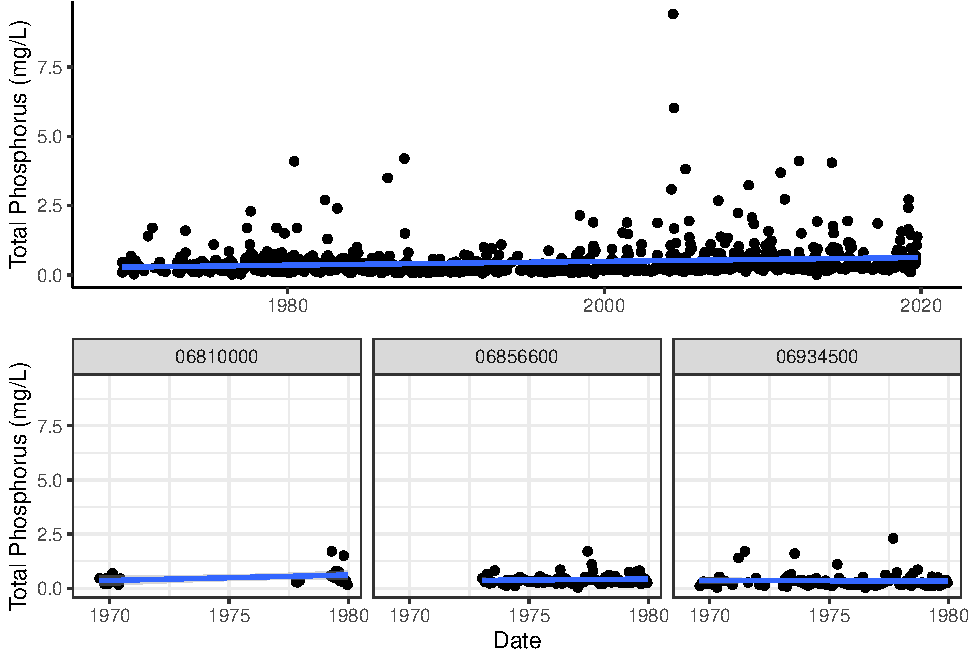
\includegraphics{Project_Template_files/figure-latex/tp.time-1.pdf}
\caption{\label{fig:tp.time}Total Phosphorus Over Time}
\end{figure}

As seen by \autoref{fig:tp.time}, total phosphorus values have a slight
positive trend. From \autoref{fig:tp.time}, site 06934500 has the most
total phosphorus data.

\begin{figure}
\centering
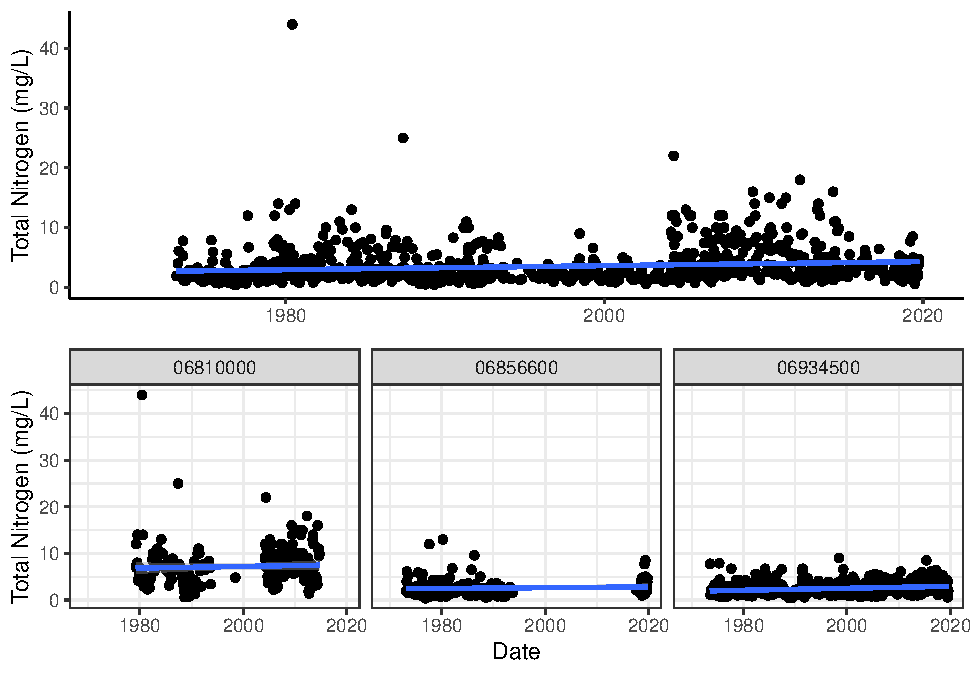
\includegraphics{Project_Template_files/figure-latex/tn.time-1.pdf}
\caption{\label{fig:tn.time}Total Nitrogen Over Time}
\end{figure}

From \autoref{fig:tn.time}, total nitrogen looks as though there is a
slight positive trend from 1980 to 2019. Again, site 06934500 has the
most total nitrogen data, as evidenced in \autoref{fig:tn.time}.

\begin{figure}
\centering
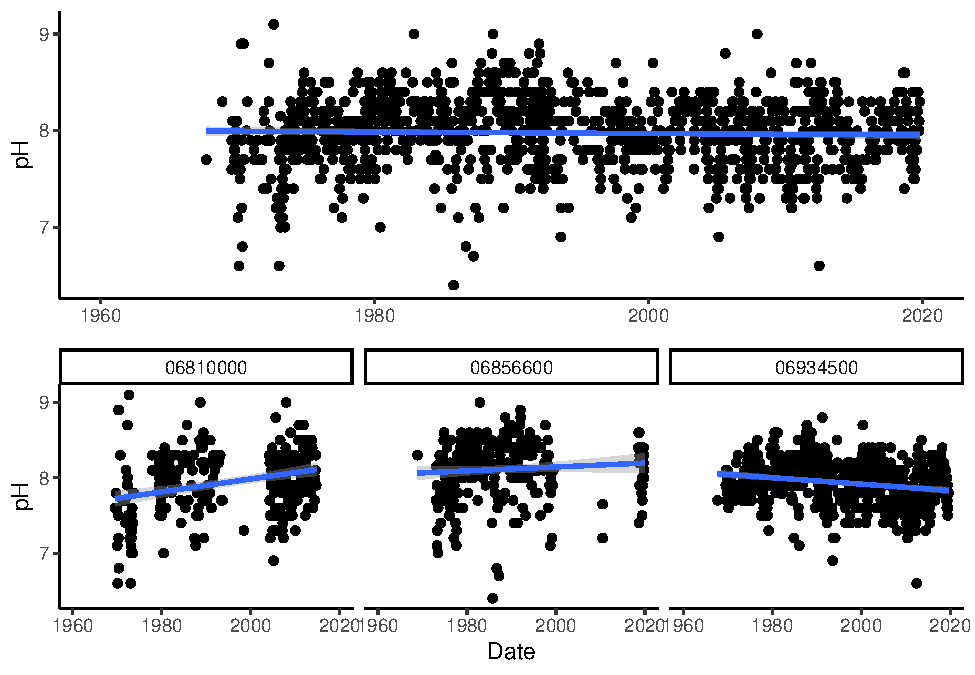
\includegraphics{Project_Template_files/figure-latex/ph-1.pdf}
\caption{\label{fig:ph}pH Over Time}
\end{figure}

As seen in \autoref{fig:ph}, pH values range from below pH of 7 to above
pH of 9 from 1970 - 2019. From \autoref{fig:ph}, site 06810000 has a
positive increase in pH over time, whereas site 06934500 has a
decreasing trend in pH over time.

\begin{figure}
\centering
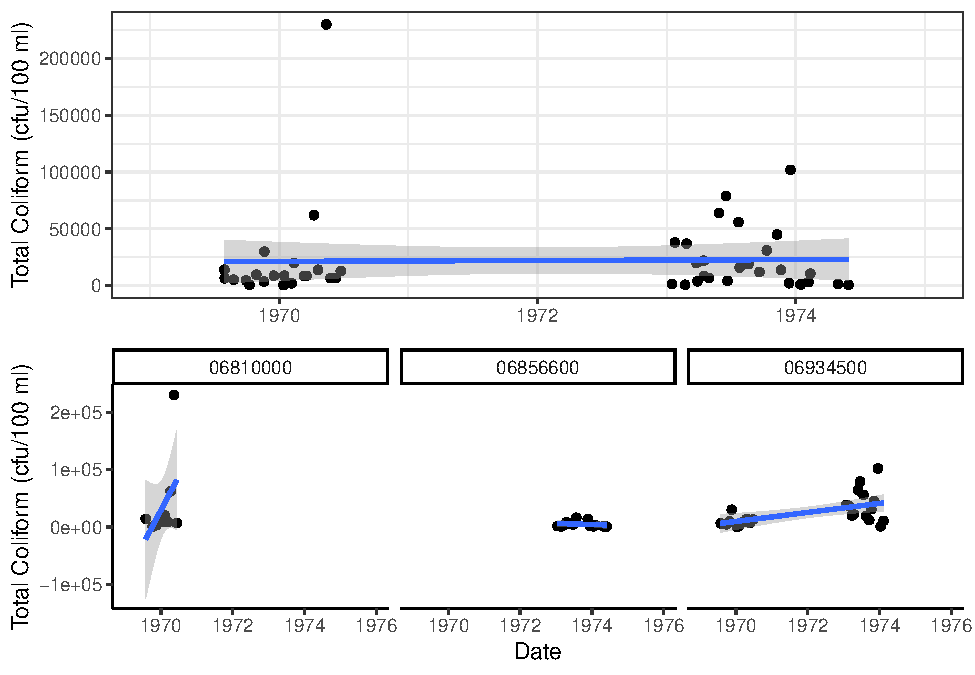
\includegraphics{Project_Template_files/figure-latex/tc.time-1.pdf}
\caption{\label{fig:tc.time}Total Coliform Over Time}
\end{figure}

\autoref{fig:tc.time} shows the total coliform measurements in the 3
chosen sites over time. From \autoref{fig:tc.time}, it is evident that
there is not much data on total coliform in the Missouri River Basin and
monitoring for total coliform occured at these 3 sites from late 1960s
through 1975.

\begin{figure}
\centering
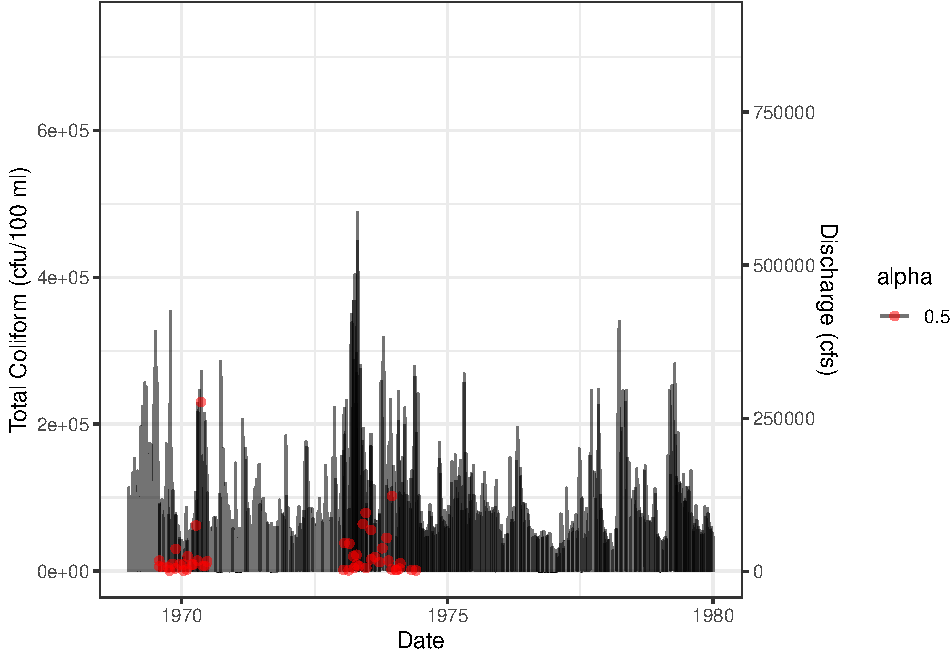
\includegraphics{Project_Template_files/figure-latex/tc.dis-1.pdf}
\caption{\label{fig:tc.dis}Total Coliform over time and Discharge over
time}
\end{figure}

\autoref{fig:tc.dis} was created to determine whether high amounts of
total coliform coincided with an increase in discharge. Because there
were limited total coliform measurements taken, as evidenced in
\autoref{fig:tc.time}, there is not a great conclusion from this data.
However, \autoref{fig:tc.dis} shows a spike in discharge events between
1972 - 1974, which also happens to be a time when total coliform was
sampled. \autoref{fig:tc.dis} also shows increases in total coliform
between 1972 - 1975.

\begin{Shaded}
\begin{Highlighting}[]
\CommentTok{#high frequency data wrangling}
\NormalTok{highfreqsite2019 <-}\StringTok{ }\NormalTok{highfreqsiteinfo }\OperatorTok
\StringTok{  }\KeywordTok{filter}\NormalTok{(end_date }\OperatorTok{>}\StringTok{ "2019-03-31"}\NormalTok{); }\KeywordTok{head}\NormalTok{(highfreqsite2019)}
\end{Highlighting}
\end{Shaded}

\begin{verbatim}
## Warning in Ops.factor(end_date, "2019-03-31"): '>' not meaningful for
## factors
\end{verbatim}

\begin{verbatim}
##  [1] X                  agency_cd          site_no           
##  [4] station_nm         site_tp_cd         dec_lat_va        
##  [7] dec_long_va        coord_acy_cd       dec_coord_datum_cd
## [10] alt_va             alt_acy_va         alt_datum_cd      
## [13] huc_cd             data_type_cd       parm_cd           
## [16] stat_cd            ts_id              loc_web_ds        
## [19] medium_grp_cd      parm_grp_cd        srs_id            
## [22] access_cd          begin_date         end_date          
## [25] count_nu          
## <0 rows> (or 0-length row.names)
\end{verbatim}

\begin{Shaded}
\begin{Highlighting}[]
\NormalTok{highfreqsites.DN <-}\StringTok{ }\KeywordTok{readNWISuv}\NormalTok{(}\DataTypeTok{site =} \KeywordTok{c}\NormalTok{(}\StringTok{"06808500"}\NormalTok{, }\StringTok{"06817000"}\NormalTok{, }\StringTok{"06892350"}\NormalTok{, }\StringTok{"06934500"}\NormalTok{), }
                               \DataTypeTok{parameterCd =} \KeywordTok{c}\NormalTok{(}\StringTok{"00060"}\NormalTok{, }\StringTok{"99133"}\NormalTok{), }
                               \CommentTok{# Discharge in cfs & Nitrate in mg/l NO3-N}
                               \DataTypeTok{startDate =} \StringTok{"2019-01-01"}\NormalTok{,}
                               \DataTypeTok{endDate =} \StringTok{"2019-11-01"}\NormalTok{) }\OperatorTok
\StringTok{                               }\KeywordTok{renameNWISColumns}\NormalTok{() }\OperatorTok
\StringTok{                               }\KeywordTok{rename}\NormalTok{(}\DataTypeTok{Nitrate_mgl =} \DecValTok{6}\NormalTok{)}

\CommentTok{#individual sites}
\NormalTok{Hermann <-}\StringTok{ }\NormalTok{highfreqsites.DN }\OperatorTok
\StringTok{           }\KeywordTok{filter}\NormalTok{(site_no}\OperatorTok{==}\StringTok{"06934500"}\NormalTok{)}
\NormalTok{Desoto <-}\StringTok{ }\NormalTok{highfreqsites.DN }\OperatorTok
\StringTok{          }\KeywordTok{filter}\NormalTok{(site_no}\OperatorTok{==}\StringTok{"06892350"}\NormalTok{)}
\NormalTok{Clarinda <-}\StringTok{ }\NormalTok{highfreqsites.DN }\OperatorTok
\StringTok{            }\KeywordTok{filter}\NormalTok{(site_no}\OperatorTok{==}\StringTok{"06817000"}\NormalTok{)}
\NormalTok{Randolph <-}\StringTok{ }\NormalTok{highfreqsites.DN }\OperatorTok
\StringTok{            }\KeywordTok{filter}\NormalTok{(site_no}\OperatorTok{==}\StringTok{"06808500"}\NormalTok{)}
\end{Highlighting}
\end{Shaded}

\hypertarget{high-frequency-nitrogen-and-discharge}{%
\subsubsection{High Frequency Nitrogen and
Discharge}\label{high-frequency-nitrogen-and-discharge}}

There were 7 sites in our region of interest that had high freq N data,
and only 4 sites had high freq N data during the floods of 2019. The
sites looked at in depth are:

\begin{verbatim}
- West Nishnabotna River in Randolph, IA
- Nodaway River at Clarinda, IA
- Kansas River in Desoto, KS
- Missouri River at Hermann, MO
\end{verbatim}

The Missouri River is the biggest river, with an average of 214693 cfs
discharge rate during the year 2019, and the Nodaway River is the
smallest river, with an average of 1185 cfs discharge rate for 2019.

In March of 2019, a
\href{https://www.kansascity.com/news/state/missouri/article228237519.html}{bomb
cyclone} hit the midwest. Our initial research question, what effect did
the March 2019 storm have on water quality, attempted to look into the
behavior of nitrogen in the discharge of the rivers. Unfortunately,
instantaneous Nitrogen values stopped recording during the peak of the
storm events in March, so it was hard to create hysteresis plots that
exhibited the type of storm and its effects on nitrogen concentration.

Even though Nitrogen concentrations were not recorded in March, they
were recorded in other times of the year. 2019 was a wet year and many
large storm events occurred.

\begin{verbatim}
## Warning: Removed 9 rows containing missing values (geom_point).
\end{verbatim}

\begin{figure}
\centering
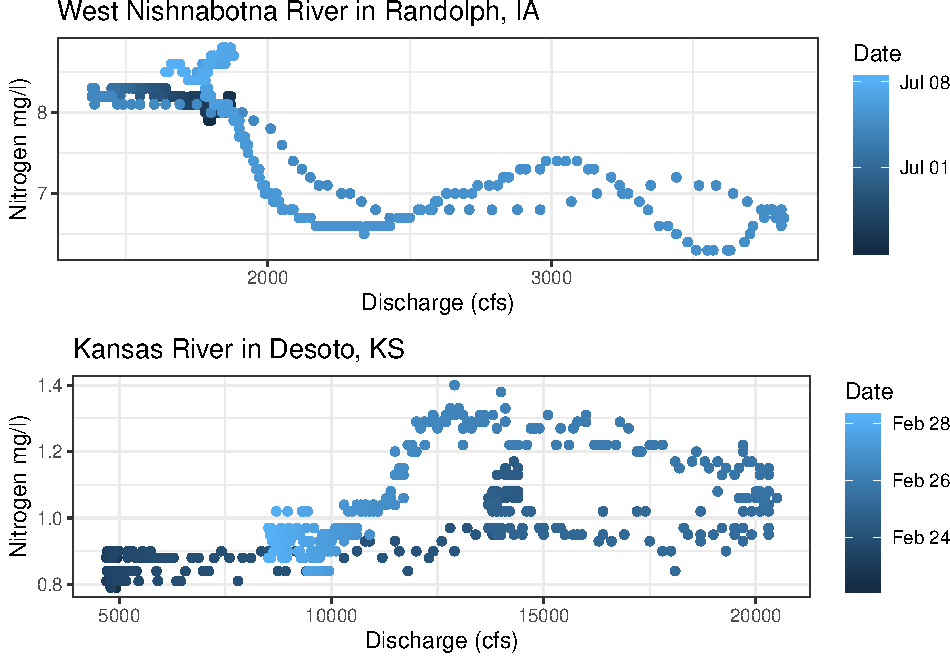
\includegraphics{Project_Template_files/figure-latex/desotos-1.pdf}
\caption{\label{fig:desotos} Hysteresis plots}
\end{figure}

The \autoref{fig:desotos} shows Hysteresis plots for two storm events in
the Missouri River Basin. The storm event on the West Nishnabotna River
exhibits an oddly-shaped plot that has a negative slope, indicating it
is a diluting storm. The Kansas River experienced a storm in late
February that has a counter-clockwise motion and a positive slope,
indicating a flushing storm. These two plots illustrate that two rivers
near each other can have very different behaviors.

\newpage

\hypertarget{analysis}{%
\section{Analysis}\label{analysis}}

\textless Include R chunks for 3+ statistical tests (display code and
output) and 3+ final visualization graphs (display graphs
only).\textgreater{}

\textless Include text sections to accompany these R chunks to explain
the reasoning behind your workflow, rationale for your approach, and the
justification of meeting or failing to meet assumptions of
tests.\textgreater{}

\newpage

\hypertarget{summary-and-conclusions}{%
\section{Summary and Conclusions}\label{summary-and-conclusions}}

\textless Summarize your major findings from your analyses. What
conclusions do you draw from your findings? Make sure to apply this to a
broader application for the research question you have
answered.\textgreater{}

\hypertarget{example-for-autoreferencing}{%
\subsection{Example for
autoreferencing}\label{example-for-autoreferencing}}

As seen by \autoref{fig:foo}, Absorbance values are not normally
distributed. This is expected, as we are dealing with ecological data.

\begin{figure}
\centering
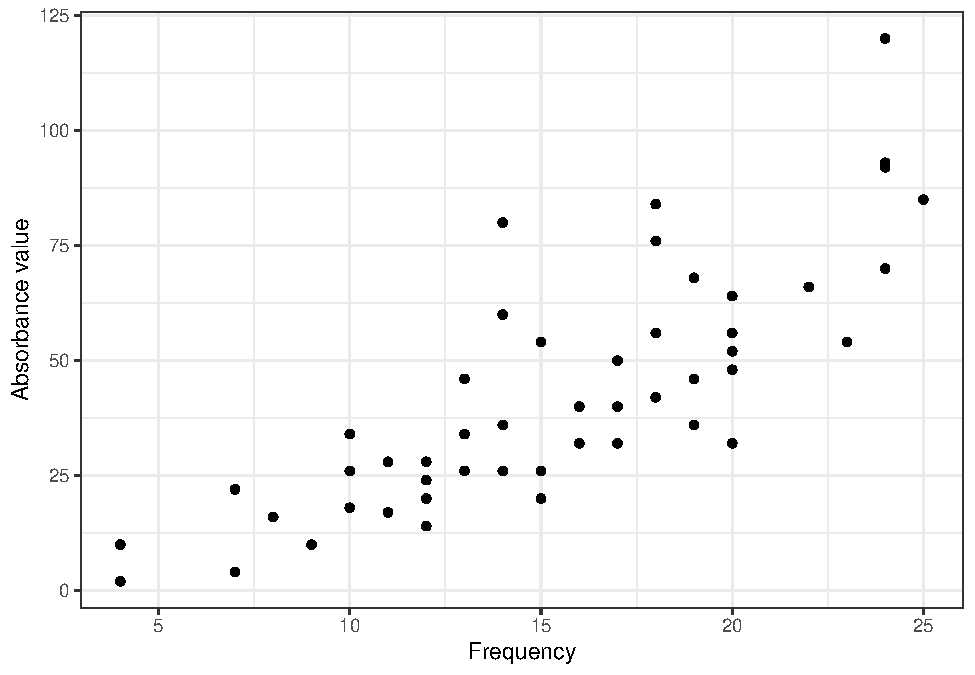
\includegraphics{Project_Template_files/figure-latex/foo-1.pdf}
\caption{\label{fig:foo}Absorbance frequency}
\end{figure}


\end{document}
